\documentclass[dvipsnames,border=5pt]{standalone}
\usepackage{tikz}
\usetikzlibrary{arrows}
\usetikzlibrary{shapes}
\usepackage{enumitem}
\usepackage{bm}
\usepackage{mathdots}
\usepackage{amsmath}
\usetikzlibrary{shadings}
\usetikzlibrary{decorations.pathreplacing}
\usepackage{helvet}
\renewcommand{\familydefault}{\sfdefault}


\usetikzlibrary{arrows,decorations.pathmorphing,backgrounds,fit,positioning,shapes.symbols,chains}
%\usepackage[top=1in, bottom=1in, left=1in, right=1.5in]{geometry}
%\def\bigsup#1{^{\vbox{\hbox{$\scriptstyle#1$}\nointerlineskip\hbox{}}}}

\begin{document}
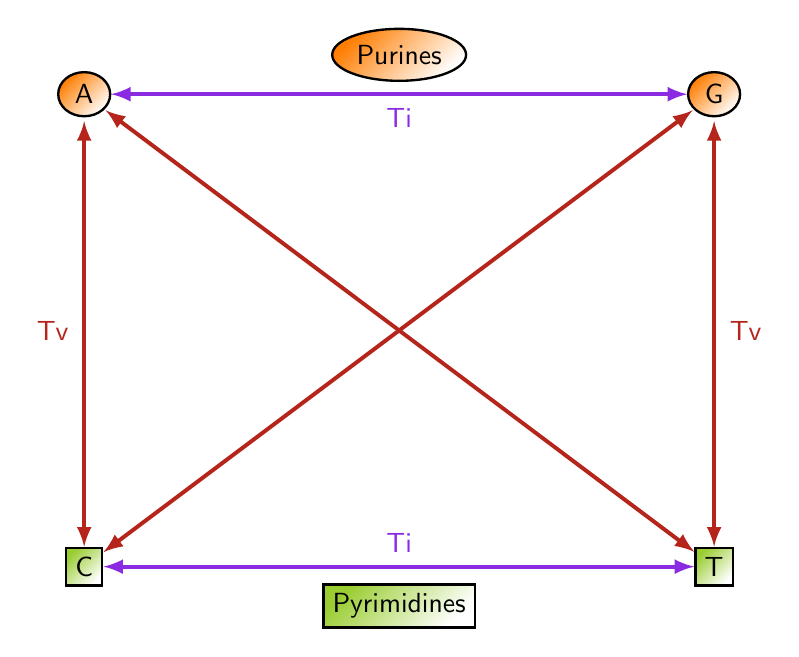
\begin{tikzpicture}
\draw [line width=0.3mm,fill=BurntOrange,left color=BurntOrange,right color=white,shading angle =45] (4,0.5) ellipse (0.85cm and 0.33cm);
\node [rectangle] at (4,0.5) (Purines) {Purines};

\draw [line width=0.3mm,fill=BurntOrange,left color=BurntOrange,right color=white,shading angle=45] (0,0) ellipse (0.33cm and 0.28cm);
\node [circle] at (0,0) (A) {A};

\draw [line width=0.3mm,fill=BurntOrange,left color=BurntOrange,right color=white,shading angle=45] (8,0) ellipse (0.33cm and 0.28cm);
\node [circle] at (8,0) (G) {G};

\node [rectangle,draw,line width=0.3mm,fill=YellowGreen,left color=YellowGreen,right color=white,shading angle=45] at (0,-6) (C) {C};

\node [rectangle,draw,line width=0.3mm,fill=YellowGreen,left color=YellowGreen,right color=white,shading angle=45] at (8,-6) (T) {T};

\node [rectangle,line width=0.3mm,draw,fill=YellowGreen,left color=YellowGreen,right color=white,shading angle=45] at (4,-6.5) (Pyrimidines) {Pyrimidines};

\draw [latex-latex,very thick,line width=0.5mm,color=BlueViolet] (A) -- (G);
\node [rectangle] at (4,-0.3) (Ti) {\textcolor{BlueViolet}{Ti}};

\draw [latex-latex,line width=0.5mm,color=BlueViolet] (C) -- (T);
\node [rectangle] at (4,-5.7) (Ti) {\textcolor{BlueViolet}{Ti}};

\draw [latex-latex,line width=0.5mm,color=BrickRed] (A) -- (T);

\draw [latex-latex,line width=0.5mm,color=BrickRed] (C) -- (G);

\draw [latex-latex,line width=0.5mm,color=BrickRed] (A) -- (C);
\node [rectangle] at (-0.4,-3) (Tv) {\textcolor{BrickRed}{Tv}};

\draw [latex-latex,line width=0.5mm,color=BrickRed] (G) -- (T);
\node [rectangle] at (8.4,-3) (Tv) {\textcolor{BrickRed}{Tv}};

\end{tikzpicture}

\end{document}
